\documentclass[12pt,letterpaper]{article}
\usepackage{preamble}

%%%%%%%%%%%%%%%%%%%%%%%%%%%%%%%%%%%%%%%%%%
%%%% Edit These for yourself
%%%%%%%%%%%%%%%%%%%%%%%%%%%%%%%%%%%%%%%%%%
\newcommand\course{CS4243}
\newcommand\hwnumber{1}
\newcommand\userID{Maximilian Fruehauf (e0445541)}

\begin{document}
\textbf{\Large CS4243 Recess Review Questions}

\section*{Question 1 Point Processing}
Matching of equations to functions:
\begin{enumerate}
	\item \( x = p + 128 \) corresponds to c).  \\
	      Since the image is simply brighter and the eyes of the child turn gray instead of black
	\item \( x = p - 128 \) corresponds to a). \\
	      Since the head of the child is completely black after the transformation (was previously \( < 128 \)).
	\item \( x = p/2 \) corresponds to b). \\
	      Since no values are absolute black (\( 0 \)) just but overall darker.
	\item \( x = 2p \) corresponds to d). \\
	      By process of elimination.
\end{enumerate}


\section*{Question 2 Linear Filtering}
\begin{enumerate}[label=(\alph*)]
	\item The \( 7\times7 \) box kernel was applied to image b), as it shows 
	      rectangular artifacts on the blurred regions, where the original image has a high contrast.
	      
	      Conversely the \( 7\times7 \) gaussian kernel as applied to image a), as it does not show 
	      these artifacts and is simply a smoother version of the original image.
	      
	\item A separable filter kernel \( k \) is one which can be split into two smaller kernels \( f,g \) as follows:
	      \begin{equation}
	      	k = f * g
	      \end{equation}
	      
	      A box filter of size 7 can be written as:
	      \begin{equation}
	      	k = \frac{1}{49} \begin{bmatrix}
	      	1 & \hdots &1 \\
	      	\vdots & \ddots & \vdots \\
	      	1 & \hdots &1 
	      	\end{bmatrix}  
	      	=
	      	\frac{1}{7} \begin{bmatrix}
	      	1 \\
	      	\vdots \\
	      	1 
	      	\end{bmatrix}
	      	*
	      	\frac{1}{7} \begin{bmatrix}
	      	1 & \hdots & 1 \\
	      	\end{bmatrix}
	      	= f * g
	      \end{equation}
\end{enumerate}


\newpage
\section*{Question 3 Corner Detection}
\begin{enumerate}[label=(\alph*)]
	\item Suitability of the functions for finding corners:
	      \begin{enumerate}
	      	\item \( R = \min(\lambda_1, \lambda_2) \) \\
	      	      If the eigenvalues \( \lambda_1, \lambda_2 \) are both large, their minimum will be as well.
	      	      This corresponds to large streching in both dimensions of \( H \), 
	      	      corresponding to a large change in the image patch in both directions.
	      	      In all other cases \( R \) is small, 
	      	      corresponding to a small change in the image patch in at least one dimension.
	      	\item \( R = \det(H) - \kappa \cdot (tr(H))^2 = \lambda_1  \lambda_2 - \kappa(\lambda_1 + \lambda_2)^2    \)  \\
	      	      If only one eigenvalue is large. Assume w.l.o.g. \( \lambda_1 \gg \lambda_2 > 0 \):
	      	      \begin{equation}
	      	      	R = 
	      	      	\lambda_1  \lambda_2 - \kappa(\lambda_1 + \lambda_2)^2
	      	      	\leq
	      	      	\lambda_1 \lambda_2 - \kappa(\lambda_1^2 + 2 \lambda_1\lambda_2)
	      	      	\approx
	      	      	-\kappa\lambda_1^2 < 0
	      	      \end{equation}
	      	      
	      	      However if \( \lambda_1 = \lambda_2 \gg 0 \):
	      	      \begin{equation}
	      	      	R = 
	      	      	\lambda_1  \lambda_2 - \kappa(\lambda_1 + \lambda_2)^2
	      	      	=
	      	      	\lambda_1^2 - 4\kappa\lambda_1^2
	      	      	\underset{\kappa < 1/4}{\approx}
	      	      	\lambda_1^2 
	      	      	> 0
	      	      \end{equation}
	      	\item \( R = \frac{\det(H)}{tr(H) + \epsilon} 
	      	      = \frac{\lambda_1 \lambda_2}{\lambda_1 + \lambda_2 + \epsilon} \) \\
	      	      If only one eigenvalue is large. Assume w.l.o.g. \( \lambda_1 \gg \lambda_2 > 0 \):
	      	      \begin{equation}
	      	      	R 
	      	      	= \frac{\lambda_1 \lambda_2}{\lambda_1 + \lambda_2 + \epsilon}
	      	      	< \frac{\lambda_1 \lambda_2}{2\lambda_1}
	      	      	= \lambda_2
	      	      \end{equation}
	      	      so \( R \in O(\lambda_2) \) and therefore small.
	      	              
	      	      However if \( \lambda_1 = \lambda_2 \gg 0 \):
	      	      \begin{equation}
	      	      	R 
	      	      	= \frac{\lambda_1 \lambda_2}{\lambda_1 + \lambda_2 + \epsilon}
	      	      	= \frac{\lambda_1^2}{2\lambda_1 + \epsilon}
	      	      	\approx \lambda_1 / 2
	      	      \end{equation}
	      	      So \( R \) is large as well.
	      \end{enumerate}
	\item the second or third function is preferable over the first one, as it represents the same notion of \"cornerness\", 
	      but does not require the expensive computation of the eigenvalues \( \lambda_1, \lambda_2 \) of \( H \).
	\item If \( \lambda_2 > k \cdot \lambda_1 \geq 0 \) with \( 0 \leq k \leq 1 \) \\
	      When gradually increasing \( k \) the constraint \( \lambda_2 > k \cdot \lambda_1 \) gradually becomes more
	      constricting until \( \lambda_2 > \lambda_1 \) for \( k = 1 \). This forces both eigenvalues 
	      to be of similar magnitude, giving a large cornerness score by the metrics above.
	      Therefore the number of corners found in an image if the constraint is fulfilled by every \( H \) matrix an image patch,
	      grows with \( k \).
\end{enumerate}


\section*{Question 4 System Design}
\begin{enumerate}[label=(\alph*)]
	\item To create a fabric fault detector, one needs to create a feature description which
	      can detect large changes in texture. For this a texton representation is suitable.
	      Here each image is processed by filters chosen from a filter bank. If the response
	      is large everywhere but small in just one spot across multiple
	      filters, this can be considered as a fault in the fabric.
	      
	      \begin{figure}[h!]
	      	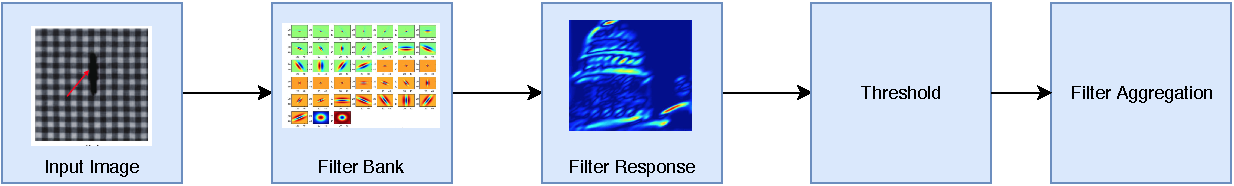
\includegraphics[width=\linewidth]{fig/filters.pdf}
	      	\caption{Fabric fault detector pipeline}
	      \end{figure}
	          
	      \begin{enumerate}
	      	\item \textbf{Input image}: Image is cropped to a fixed size.
	      	\item \textbf{Filter Bank}: Each filter of the filter bank is convolved with the image.
	      	\item \textbf{Filter Response}: For each of the filters, a response map is created, which is
	      	      a normalized value, of how much the image in the given window matches the filter kernel.
	      	\item \textbf{Threshold}: A threshold is applied on every filter response pixel value \( p \)
	      	      in the form of \( p' = \min(p, \tau_i) \), where \( \tau_i \) is the maximal response allowed for each filter kernel \( \kappa_i \).
	      	\item \textbf{Filter Aggregation}: The responses for each of the filters is collected 
	      	      after applying the threshold and if a certain set of filter responses show a low enough
	      	      response in local image patches, the image is marked as a faulty fabric.
	      \end{enumerate}
	      
	      When training this algorithm, the goal is to identify the set of filter kernels
	      in the aggregation step, which when giving a low response correspond to a faulty fabric.
	      
	\item For detecting each of the faults in the given images, 
	      the Threshold and aggregation sections of the classifier needs to be fitted to
	      make sure they are classified as faulty. Therefore these images are used as training examples.
\end{enumerate}
\end{document}